\documentclass{beamer}

\usepackage{amsmath}
\usepackage{hyperref}
\usepackage{dsfont}
\usepackage{pythonhighlight}

\hypersetup{
    colorlinks=true,
    linkcolor=blue,
    filecolor=magenta,      
    urlcolor=cyan
}


% macros
\newcommand{\N}{\mathbb{N}}
\newcommand{\Z}{\mathbb{Z}}
\newcommand{\R}{\mathbb{R}}
\newcommand{\Q}{\mathbb{Q}}
\newcommand{\Ha}{\mathbb{H}}
\newcommand{\C}{\mathbb{C}}

\DeclareMathOperator*{\argmax}{argmax}
\DeclareMathOperator*{\argmin}{argmin}


\usetheme{metropolis}   

\title{SQL For Data Analysis}
\subtitle{A Language for Querying Structured Data}
\author{Anders Poirel}
\institute{Data Science @ SC}

\logo{
\includegraphics[height=0.75cm]{figures/improved-logo.png}}

\begin{document}

\maketitle

    \begin{frame}{SQL}
        \begin{itemize}
            \item language for querying \alert{structured data}
            \item \alert{structured} data: data in row-column form where each row corresponds to a datapoint
            \item each database is composed of several \alert{tables} with the above structure
            \item SQL is standardized but most implementations aren't compliant
        \end{itemize}   
    \end{frame}


    \begin{frame}{SQLite}
        \begin{itemize}
            \item A lightweight database using static files on a disk
            \item Good for prototyping a database before switching to something more complicated if needed
            \item In practice use \alert{SQL Alchemy} to make code more portable between databases
        \end{itemize}   
    \end{frame}
    
    \begin{frame}[fragile]{Select queries}
    
        Structure of a \alert{SELECT} query:
        \begin{verbatim}
        SELECT DISTINCT column, AGG_FUNC(column), ...
        FROM mytable
            JOIN anothertable
            ON mytable.column = anothertable.column
        WHERE expression
        GROUP BY column
        HAVING expression
        ORDER BY column ASC/DESC 
        LIMIT count OFFSET count
        \end{verbatim}

    \end{frame}

    \begin{frame}[fragile]{Select}

        To select a \alert{particular} column,
        \begin{verbatim}
        SELECT (DISTINCT) column
        FROM mytable
        \end{verbatim}

        To select \alert{all} columns,
        \begin{verbatim}
        SELECT *
        FROM mytable
        \end{verbatim}

    \end{frame}


    \begin{frame}[fragile]{Select Constraints (1)}

        To \alert{constrain} the output of SELECT,
        \begin{verbatim}
        SELECT column1, ... 
        WHERE 
            condition1
            AND/OR condition2 ...
        \end{verbatim}
    \end{frame}

    
    \begin{frame}[fragile]{Select Constraints (2)}
        Common operators in WHERE Expressions:
        \begin{itemize}
            \item =, !=, <, >, <=, >=
            \item BETWEEN ... AND ..
            \item NOT BETWEEN ... AND ..
            \item LIKE
            \item NOT LIKE
            \item \%adcd\%
            \item IN (...)
            \item NOT IN (...)
        \end{itemize}
    \end{frame}

    \begin{frame}[fragile]{Joins (1)}
        To \alert{merge} two tables based on a unique identifer,
        \begin{verbatim}
            SELECT column, ...
            FROM mytable
            INNER/LEFT/RIGHT/FULL JOIN anothertable
                ON mytable.id = anothertable.id
        \end{verbatim}
    \end{frame}
    
    \begin{frame}{Joins (2)}
        \begin{center}
            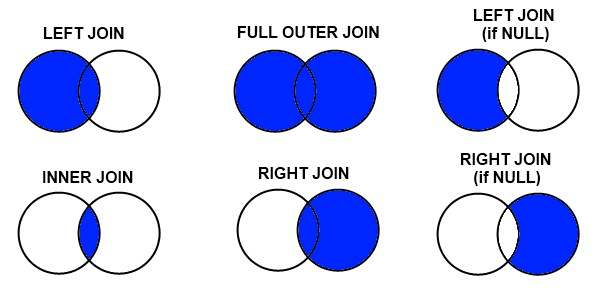
\includegraphics[width=0.8\textwidth]{figures/joins.jpg}
        \end{center}
    \end{frame}


    \begin{frame}[fragile]{Sorting}
        To \alert{sort} based on a column
        \begin{verbatim}
        SELECT column, ...
        FROM mytable
        ORDER BY column ASC/DESC
        \end{verbatim}
    \end{frame}

    
    \begin{frame}[fragile]{Aggregates (1)}
        To \alert{aggregate} by category,
        \begin{verbatim}
        SELECT AGG_FUNC(column)
        WHERE expression
        GROUP BY column
        HAVING expression
        \end{verbatim}
    \end{frame}


    \begin{frame}[fragile]{Aggregates (2)}
        Common aggregates:
        \begin{itemize}
            \item AVG
            \item SUM
            \item MIN 
            \item MAX
        \end{itemize}
    \end{frame}

    \begin{frame}[fragile]{Select Queries Recap}
    
        \begin{verbatim}
        SELECT DISTINCT column, AGG_FUNC(column), ...
        FROM mytable
            JOIN anothertable
            ON mytable.column = anothertable.column
        WHERE expression
        GROUP BY column
        HAVING expression
        ORDER BY column ASC/DESC 
        LIMIT count OFFSET count
        \end{verbatim}

    \end{frame}


\end{document}